\section{Implementation}
\label{sec:Aufbau}

\subsection{Setup}
For this experiment, which is used to determine the molar heat capacity of copper, the apparatus shown in \autoref{fig:Aufbau} is needed.
\begin{figure}
    \centering
        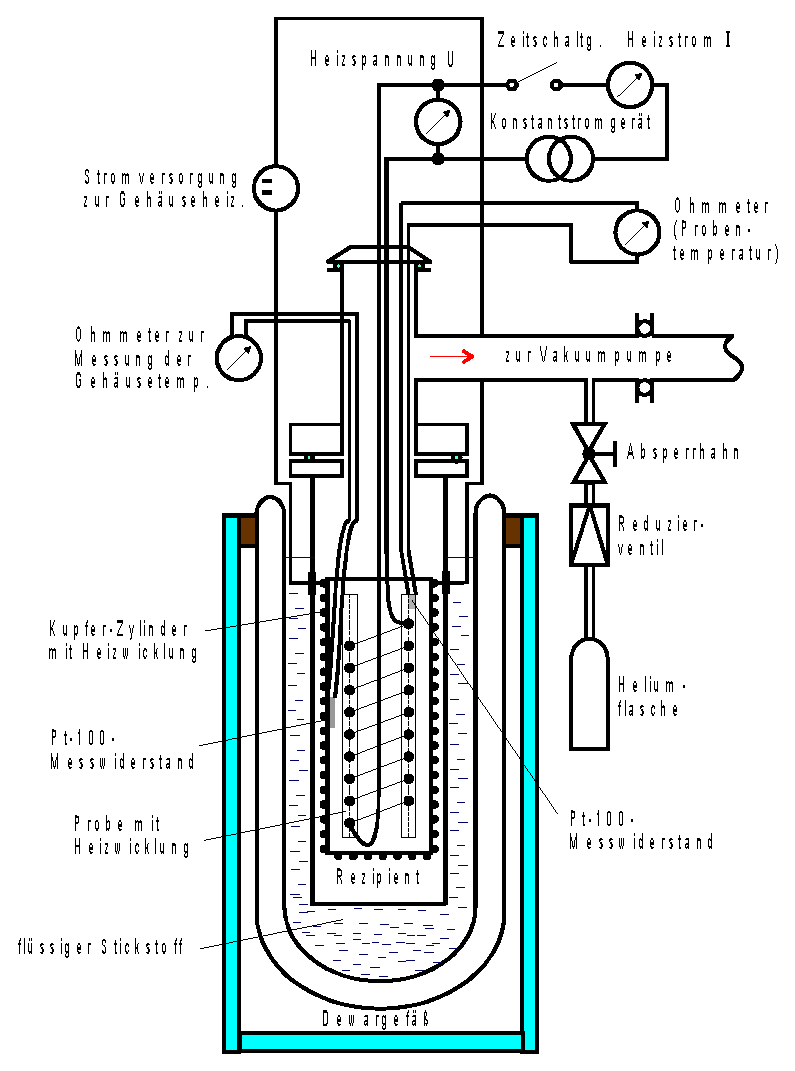
\includegraphics[width=0.5\textwidth]{Aufbau.pdf}
        \caption{Simplified representation of the used apparatus \cite{ap47}.}
        \label{fig:Aufbau}
\end{figure}
The heart of this setup is the with liquid nitrogen filled Dewar vessel. The copper cylinder is placed inside of it. In order to be in control of the samples's temperature, it is surrounded by a heating coil.
The temperature is measured by two PT-100 measuring resistors whose electrical resistant changes monotonically with temperature.
The mathematical equation that puts resistance and temperature in relation is given by 
\begin{equation*}
    T=0.00134 R^2+2.296-243.02+274.15\; . 
\end{equation*}
The recipient is connected to a vacuum pump and a helium supply during cooling. Both sample and cylinder are supplied with a heating voltage.


\subsection{Measurement method}
The first step is to evacuate the recipient to prevent the liquefaction of air in the cylinder due to low temperatures.
Secondly, helium is filled in because it does not liquify at temperatures about $T=80\, \unit{\kelvin}$. Further helium has a good thermal conductivity.
As mentioned the temperature to start with is $T=80\, \unit{\kelvin}$, when T is reached the recipient is evacuated again to reduce pressure even further and decrease loss due to conductivity, evaporation and radiation.
Then energy in form of heat (by increasing the heating voltage) is put into the system which leads to a rise in temperature.  
The $\Delta T$ is supposed to be between $7-11\,\unit{\kelvin} $ to prevent exalted heat loss due to a high temperature gradient.
Afterwards, the copper cylinder is heated to the same temperature as the recipient.
To determine the molar heat capacity of copper between  $T=80\, \unit{\kelvin}$ and $T=300\, \unit{\kelvin}$, temperature needs to be gradually increased while measuring time, voltage and heating current are recorded.
Important: Presssure is kept at atmospheric pressure during the duration of the measurement.